\section{Landasan Aljabar Abstrak}
\label{sec:aljabar-abstrak}

Kriptografi Kurva Eliptik bertumpu pada satu gagasan yang tidak biasa: alih-alih
menghitung dengan bilangan bulat raksasa sebagaimana RSA dan ElGamal, ia
menghitung dengan \emph{titik-titik} pada sebuah kurva. Agar titik-titik itu
dapat dijumlahkan, dikurangkan, dan dikalikan dengan bilangan bulat secara
konsisten, himpunan titik tersebut harus membentuk struktur aljabar yang
tertutup dan teratur. Struktur itulah yang menjadi pokok bahasan bagian ini.

Sebelum satu persamaan kurva pun ditulis, pembaca perlu memegang tiga perkakas
aljabar: \textbf{grup}, \textbf{medan}, dan \textbf{medan berhingga}. Ketiganya
bukan hiasan teoretis. Sifat-sifat yang diperiksa di sini --- mengapa sebuah
operasi selalu menghasilkan elemen di dalam himpunan yang sama, mengapa setiap
elemen punya lawan, dan mengapa pembagian selalu boleh dilakukan --- justru
sifat-sifat yang menjamin bahwa enkripsi kurva eliptik dapat dibalik oleh
penerima yang sah tetapi tidak oleh penyadap.

\subsection{Grup dan Keempat Aksiomanya}
\label{subsec:grup}

Sebuah \textbf{grup} (\textit{group}) adalah sistem aljabar yang terdiri atas
sebuah himpunan $G$ bersama sebuah operasi biner $*$ yang memetakan setiap
pasangan elemen $G$ kembali ke $G$. Pasangan itu ditulis $\langle G, * \rangle$.
Supaya layak disebut grup, untuk semua $a, b, c \in G$ harus berlaku keempat
aksioma berikut.

\begin{enumerate}
    \item \textbf{Ketertutupan} (\textit{closure}): $a * b \in G$. Operasi tidak
          pernah menghasilkan elemen di luar himpunan.
    \item \textbf{Asosiatif}: $a * (b * c) = (a * b) * c$. Pengelompokan tidak
          mengubah hasil, sehingga rangkaian operasi boleh dihitung dari arah
          mana pun.
    \item \textbf{Elemen netral}: terdapat $e \in G$ sedemikian sehingga
          $a * e = e * a = a$ untuk setiap $a$. Elemen ini bersifat tunggal.
    \item \textbf{Elemen invers}: untuk setiap $a \in G$ terdapat $a' \in G$
          sedemikian sehingga $a * a' = a' * a = e$.
\end{enumerate}

Perhatikan bahwa aksioma keempat menyatakan sesuatu yang lebih kuat daripada
yang tampak. Ia tidak sekadar mengatakan bahwa setiap elemen \emph{punya}
lawan, melainkan bahwa lawan itu \emph{berada di dalam himpunan yang sama}.
Himpunan bilangan asli $\N$ dengan operasi penjumlahan memenuhi ketiga aksioma
pertama, tetapi gagal pada aksioma keempat: lawan dari $3$ adalah $-3$, dan $-3$
tidak termasuk himpunan bilangan asli. Karena itu $\langle \N, + \rangle$
bukanlah grup. Keadaan itu penting bagi kriptografi, sebab sebuah operasi
enkripsi hanya dapat dibalik bila inversnya tersedia di dalam himpunan yang
sama dengan tempat pekerjaan itu berlangsung.

Notasi $\langle G, + \rangle$ menandai grup dengan operasi penjumlahan,
sedangkan $\langle G, \cdot \rangle$ menandai grup dengan operasi perkalian.
Tabel~\ref{tab:contoh-grup} memuat contoh-contoh yang akan dipakai berulang
kali di sepanjang bab ini.

\begin{table}[htbp]
    \centering
    \caption{Contoh-contoh grup dan pemeriksaan aksioma inversnya}
    \label{tab:contoh-grup}
    \begin{tabularx}{\linewidth}{@{}l c c l
                                   >{\raggedright\arraybackslash}X@{}}
    \toprule
    \textbf{Himpunan} & \textbf{Operasi} & \textbf{$e$} & \textbf{$a'$} &
    \textbf{Keterangan} \\
    \midrule
    $\langle \R, + \rangle$ & $+$ & $0$ & $-a$ &
    Grup abelian; lawan selalu ada di dalam $\R$ \\
    \addlinespace
    $\langle \R^*, \cdot \rangle$ & $\cdot$ & $1$ & $1/a$ &
    Grup abelian; $\R^* = \R - \{0\}$, sebab $1/0$ tidak terdefinisi \\
    \addlinespace
    $\langle \Z, + \rangle$ & $+$ & $0$ & $-a$ &
    Grup abelian; bilangan bulat negatif tetap di dalam $\Z$ \\
    \addlinespace
    $\langle \Z, \cdot \rangle$ & $\cdot$ & $1$ & --- &
    \textbf{Bukan grup}: hanya $1$ dan $-1$ yang punya invers di dalam $\Z$,
    sebab $2 \cdot a' = 1$ tidak punya jawaban bulat \\
    \addlinespace
    $\langle \Z_n, \oplus \rangle$ & $\oplus$ & $0$ & $n - a$ &
    Grup abelian; $\oplus$ berarti penjumlahan modulo $n$ \\
    \addlinespace
    $\langle \Z_p^*, \otimes \rangle$ & $\otimes$ & $1$ & $a^{-1}$ &
    Grup abelian dengan $p$ prima; invers selalu ada berkat Teorema Euler
    (Bab~\ref{chap:landasan-matematika}) \\
    \bottomrule
    \end{tabularx}
\end{table}

Baris keempat pada Tabel~\ref{tab:contoh-grup} sering luput dari pemeriksaan.
Himpunan bilangan bulat dengan operasi perkalian memang tertutup, asosiatif,
dan memiliki elemen netral $1$; yang tidak dimilikinya adalah invers. Elemen
$5$ tidak punya lawan perkalian di dalam $\Z$, sebab tidak ada bilangan bulat
$a'$ dengan $5 \cdot a' = 1$. Karena itu $\langle \Z, \cdot \rangle$ hanya
sebuah \emph{monoid}, bukan grup. Perbedaan ini akan kembali muncul pada
Subbagian~\ref{subsec:medan}, ketika sifat yang sama menentukan apakah suatu
himpunan layak disebut medan.

\subsection{Grup Abelian}
\label{subsec:grup-abelian}

Sebuah grup $\langle G, * \rangle$ disebut \textbf{grup komutatif} atau
\textbf{grup abelian} bila aksioma kelima dipenuhi, yaitu
\[ a * b = b * a \quad \text{untuk semua } a, b \in G . \]
Istilah \emph{abelian} diambil dari nama Niels Henrik Abel (1802--1829),
matematikawan Norwegia yang meninggal pada usia dua puluh enam tahun. Nama itu
dipakai untuk menghormati hasilnya yang paling terkenal: bukti lengkap pertama
bahwa persamaan berderajat lima tidak dapat diselesaikan dengan rumus akar,
persoalan yang telah terbuka selama dua setengah abad. Abel juga meletakkan
dasar teori fungsi eliptik --- cabang matematika yang namanya kini dipinjam
oleh kurva yang menjadi pokok bab ini \citep{stallings2017}.

Keempat contoh pertama pada Tabel~\ref{tab:contoh-grup} bersifat abelian,
demikian pula kedua contoh terakhirnya, sebab baik penjumlahan modulo $n$
maupun perkalian modulo prima selalu dapat ditukar urutannya. Sebaliknya,
himpunan matriks $2 \times 2$ berdeterminan tidak nol dengan operasi perkalian
matriks \emph{bukan} grup abelian. Alasannya terletak pada aturan perkalian
matriks: baris dikalikan dengan kolom, sehingga menukar posisi kedua faktor
mengubah cara setiap elemen dihitung. Sebagai contoh,
\[
\begin{pmatrix} 1 & 1 \\ 0 & 1 \end{pmatrix}
\begin{pmatrix} 1 & 0 \\ 1 & 1 \end{pmatrix}
=
\begin{pmatrix} 2 & 1 \\ 1 & 1 \end{pmatrix},
\qquad
\begin{pmatrix} 1 & 0 \\ 1 & 1 \end{pmatrix}
\begin{pmatrix} 1 & 1 \\ 0 & 1 \end{pmatrix}
=
\begin{pmatrix} 1 & 1 \\ 1 & 2 \end{pmatrix}.
\]
Kedua hasilnya berbeda, jadi urutan perkalian benar-benar berpengaruh.

Sifat komutatif bukan kemewahan. Di dalam ECC, pertukaran kunci ECDH bekerja
justru karena $ab = ba$: Alice dan Bob menghitung perkalian skalar dengan
urutan yang berbeda, dan keduanya harus memperoleh titik yang sama. Tanpa
komutativitas, pertukaran kunci kurva eliptik tidak mungkin dirancang.

\subsection{Medan}
\label{subsec:medan}

Sebuah \textbf{medan} (\textit{field}) adalah sistem aljabar yang terdiri atas
sebuah himpunan $F$ bersama \emph{dua} operasi biner, yaitu penjumlahan $(+)$
dan perkalian $(\cdot)$. Struktur $\langle F, +, \cdot \rangle$ disebut medan
jika dan hanya jika ketiga syarat berikut dipenuhi.

\begin{enumerate}
    \item $\langle F, + \rangle$ adalah grup abelian.
    \item $\langle F - \{0\}, \cdot \rangle$ adalah grup abelian. Perhatikan
          bahwa elemen nol dikeluarkan lebih dahulu; sebab bila tidak, syarat
          ketiga akan gugur.
    \item Operasi perkalian menyebar (\textit{distributive}) terhadap operasi
          penjumlahan:
          \[
          \begin{aligned}
          x \cdot (y + z) &= (x \cdot y) + (x \cdot z), \\
          (x + y) \cdot z &= (x \cdot z) + (y \cdot z) .
          \end{aligned}
          \]
\end{enumerate}

Ketiga syarat itu menuntut lebih banyak daripada syarat grup. Bukan saja
setiap elemen harus punya lawan penjumlahan, melainkan setiap elemen bukan nol
harus punya \emph{lawan perkalian}. Akibatnya pembagian selalu dapat dilakukan,
dan itulah yang membuat rumus gradien pada Bab~\ref{chap:ecc} --- yang selalu
berbentuk pecahan --- dapat dikerjakan sepenuhnya di dalam himpunan. Medan juga
mewarisi seluruh aksioma grup: ketertutupan, komutatif, asosiatif, elemen
netral, elemen invers, dan distributif.

\begin{table}[htbp]
    \centering
    \caption{Himpunan bilangan dan statusnya sebagai medan}
    \label{tab:contoh-medan}
    \begin{tabularx}{\linewidth}{@{}l l
                                   >{\raggedright\arraybackslash}X@{}}
    \toprule
    \textbf{Struktur} & \textbf{Status} & \textbf{Alasan} \\
    \midrule
    $\langle \mathbb{Q}, +, \cdot \rangle$ & Medan &
    Setiap pecahan bukan nol $p/q$ punya kebalikan $q/p$ yang juga pecahan \\
    \addlinespace
    $\langle \R, +, \cdot \rangle$ & Medan &
    Kebalikan setiap bilangan riil bukan nol adalah bilangan riil \\
    \addlinespace
    $\langle \Z, +, \cdot \rangle$ & \textbf{Bukan medan} &
    $\langle \Z, + \rangle$ memang grup abelian, tetapi
    $\langle \Z - \{0\}, \cdot \rangle$ bukan grup: kebalikan $2$ adalah
    $1/2$, yang bukan bilangan bulat \\
    \addlinespace
    $\langle \Z_n, +, \cdot \rangle$ & Medan hanya bila $n$ prima &
    Kebalikan $a$ modulo $n$ ada tepat ketika $\text{PBB}(a, n) = 1$; untuk
    $n = 6$ elemen $2$ dan $3$ tidak punya kebalikan \\
    \addlinespace
    $\langle \Z_p, +, \cdot \rangle$ & Medan, dengan $p$ prima &
    Setiap $a \in \{1, \dots, p-1\}$ koprima dengan $p$, sehingga kebalikannya
    selalu ada \\
    \bottomrule
    \end{tabularx}
\end{table}

Pelajaran dari Tabel~\ref{tab:contoh-medan} adalah bahwa jumlah elemen yang
tak berhingga tidak menjamin adanya medan, dan sebaliknya jumlah elemen yang
berhingga tidak menghalanginya. Bilangan bulat $\Z$ yang jauh lebih kaya
daripada $\Z_p$ justru gagal menjadi medan, sementara $\Z_p$ yang hanya berisi
$p$ elemen berhasil. Yang menentukan bukan luasnya himpunan, melainkan apakah
setiap elemen bukan nol punya kebalikan di dalam himpunan itu.

\subsection{Medan Berhingga dan Medan Galois}
\label{subsec:medan-berhingga}

Sebuah medan disebut \textbf{medan berhingga} (\textit{finite field}) bila
himpunan elemennya berhingga. Bila banyaknya elemen adalah $n$, notasinya
adalah $F_n$. Contoh paling kecil adalah $F_2 = \{0, 1\}$, medan dengan dua
elemen: penjumlahan dan perkaliannya adalah aritmetika modulo $2$, sehingga
$1 + 1 = 0$.

Medan berhingga juga dinamai \textbf{Medan Galois} (\textit{Galois Field}),
untuk menghormati Évariste Galois (1811--1832), matematikawan Prancis yang
meninggal pada usia dua puluh tahun dan meninggalkan dasar teori grup serta
teori persamaan yang menjadi tulang punggung aljabar modern. Notasi
$GF(p^m)$ menandai medan berhingga dengan $p^m$ elemen, dengan $p$ prima dan
$m \ge 1$. Kasus paling sederhana terjadi ketika $m = 1$, sehingga
$GF(p)$ --- sering pula ditulis $F_p$ --- berisi himpunan
$\{0, 1, \dots, p-1\}$ dengan penjumlahan dan perkalian dilakukan modulo $p$.

Contoh paling ringkas adalah $GF(23)$, medan berhingga dengan dua puluh tiga
elemen. Operasi di dalamnya mengikuti aturan yang sama dengan aritmetika jam:
hasil dihitung seperti biasa, lalu dikurangi kelipatan $23$ sampai sisanya
berada di dalam $\{0, 1, \dots, 22\}$. Karena itu
\[
12 + 20 = 32 \equiv 9 \pmod{23}
\qquad \text{dan} \qquad
8 \cdot 9 = 72 \equiv 3 \pmod{23} .
\]
Yang kedua menarik untuk dicermati: hasil perkaliannya justru \emph{lebih
kecil} daripada kedua faktornya. Perilaku semacam itu tidak mungkin terjadi
pada bilangan bulat biasa, dan ia langsung terlihat begitu modulus dipakai.

Perkalian modulo prima juga memberi cara mencari akar kuadrat yang tidak
tersedia di bilangan bulat. Misalkan dicari penyelesaian $x^2 \equiv 5
\pmod{11}$. Karena hanya ada sebelas kandidat, seluruhnya dapat diperiksa
sekali jalan: kuadrat dari $0, 1, \dots, 10$ modulo $11$ berturut-turut adalah
$0, 1, 4, 9, 5, 3, 3, 5, 9, 4, 1$. Nilai $5$ muncul dua kali, yaitu pada $x = 4$
dan $x = 7$. Jadi
\begin{equation}
x^2 \equiv 5 \pmod{11}
\quad\Longrightarrow\quad
x_1 = 4 \quad \text{atau} \quad x_2 = 7 .
\label{eq:akar-gf11}
\end{equation}
Perhatikan bahwa $5$ yang diambil akar kuadratnya tidak punya akar kuadrat
dalam bilangan bulat, sedangkan di dalam $GF(11)$ ia punya dua akar sekaligus.
Gambar~\ref{fig:tabel-gf11} memperlihatkan tabel perkalian $GF(11)$ lengkap
beserta penandaan kedua akar tersebut.

\begin{figure}[htbp]
    \centering
    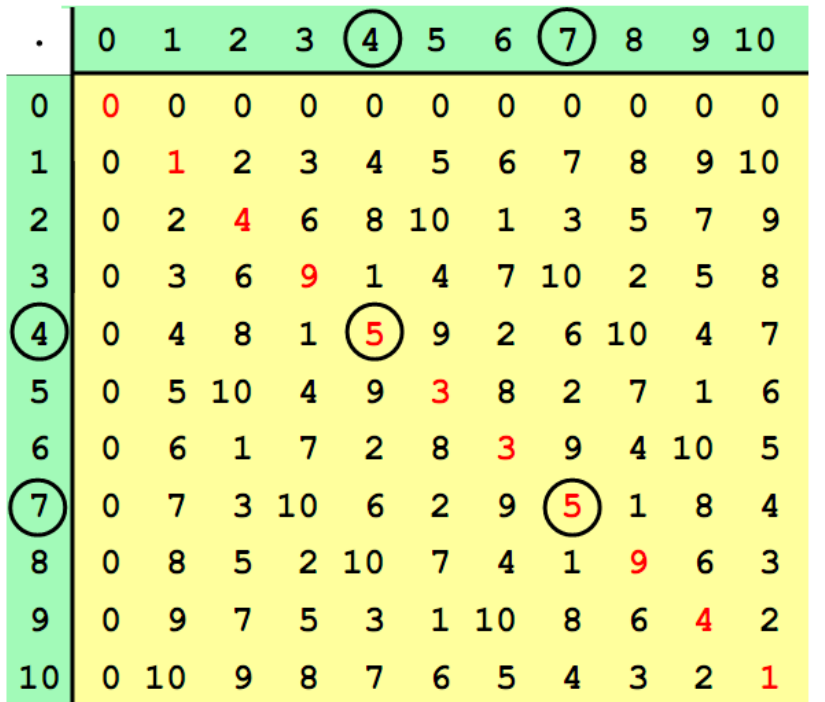
\includegraphics[width=0.55\linewidth, height=0.65\textheight, keepaspectratio]{figures/tabel-gf11.png}
    \caption{Tabel perkalian $GF(11)$. Kotak bertanda menandai nilai $5$ pada
    diagonal, dan elemen mendatar atau tegaknya --- $x = 4$ serta $x = 7$ ---
    adalah penyelesaian $x^2 \equiv 5 \pmod{11}$ pada
    Persamaan~\eqref{eq:akar-gf11}}
    \label{fig:tabel-gf11}
    \sumber{Andreas Steffen, \textit{Elliptic Curve Cryptography}, melalui
    Munir, \textit{IF4020 Kriptografi}, ITB.}
\end{figure}

Keberadaan dua akar itu bukan kebetulan, melainkan tanda bahwa $5$ adalah
residu kuadratik di dalam $GF(11)$. Pada ranah kriptografi, sifat inilah yang
nanti dipakai oleh metode Koblitz untuk mengubah pesan menjadi titik kurva:
penyandi mencoba sederet nilai $x$ sampai ia menemukan satu yang membuat ruas
kanan kurva menjadi residu kuadratik, lalu mengambil akar kuadratnya sebagai
koordinat $y$ (Bagian~\ref{sec:implementasi-ecc}).

\subsection{Aritmetika Polinomial di dalam Medan Biner}
\label{subsec:gf-2m}

Dari $GF(p^m)$, kasus $p = 2$ mendapat perlakuan khusus karena komputernya
bekerja dengan bit. Medan $GF(2^m)$ --- disebut juga medan berhingga biner ---
adalah ruang vektor berdimensi $m$ atas $GF(2)$. Setiap elemen di dalamnya
adalah bilangan bulat dengan representasi biner paling banyak $m$ bit, dan
setiap rangkaian bit dapat dipandang sebagai sebuah polinom dengan suku banyak
maksimal $m$ dan koefisien di dalam $GF(2)$. Rangkaian bit
$b_{m-1}b_{m-2}\dots b_1b_0$ menyatakan polinom
\begin{equation}
b_{m-1}x^{m-1} + b_{m-2}x^{m-2} + \dots + b_1x + b_0 .
\label{eq:gf2m-polinom}
\end{equation}
Karena itu, misalnya, empat bit $1101$ di dalam $GF(2^4)$ menyatakan polinom
$x^3 + x^2 + 1$.

Penjumlahan dua elemen $GF(2^m)$ dilakukan suku demi suku dengan koefisien
dijumlahkan modulo $2$:
\begin{equation}
a + b = c, \qquad c_i = (a_i + b_i) \bmod 2 .
\label{eq:gf2m-tambah}
\end{equation}
Karena $0 + 0 = 0$, $1 + 0 = 1$, dan $1 + 1 = 0$, seluruh tabel penjumlahannya
tidak lain adalah operasi \textbf{XOR} bit demi bit. Sifat itu membuat
penjumlahan di dalam $GF(2^m)$ sangat murah untuk diimplementasikan: satu
instruksi mesin, tanpa penyimpanan, tanpa pengambilan modulo.

Sebagai contoh pertama, ambil $a = \code{00001101} = x^3 + x^2 + 1$ dan
$b = \code{00000110} = x^2 + x$, keduanya di dalam $GF(2^8)$. Dalam notasi
heksadesimal keduanya ditulis $a = \text{'0D'}$ dan $b = \text{'06'}$. Menurut
Persamaan~\eqref{eq:gf2m-tambah},
\[
a + b = (x^3 + x^2 + 1) + (x^2 + x) = x^3 + 2x^2 + x + 1 .
\]
Koefisien $2x^2$ diambil modulo $2$, sehingga menjadi $0x^2$:
\[
a + b = x^3 + x + 1 = \code{00001011} = \text{'0B'} .
\]
Cara yang sama berlaku untuk contoh kedua, $a = \code{01010111} =
x^6 + x^4 + x^2 + x + 1$ dan $b = \code{10000011} = x^7 + x + 1$. Dalam notasi
heksadesimal keduanya adalah $a = \text{'57'}$ dan $b = \text{'83'}$, dan
hasilnya
\[
a + b = x^7 + x^6 + x^4 + x^2 + x = \code{11010100} = \text{'D4'} .
\]
Perhatikan bahwa kedua contoh itu dapat diselesaikan jauh lebih cepat dengan
meng-XOR-kan langsung kedua bilangan heksadesimalnya:
$0\text{D} \oplus 06 = 0\text{B}$ dan $57 \oplus 83 = \text{D4}$.

Perkalian tidak sesederhana penjumlahan, sebab hasil kali dua polinom
berderajat tinggi dapat melewati batas $m$ bit. Hasil kalinya didefinisikan
sebagai sisa pembagian perkalian kedua polinom itu oleh sebuah polinom
tereduksi berderajat $m$:
\begin{equation}
a \cdot b = c, \qquad c \equiv a(x) \cdot b(x) \pmod{f(x)} ,
\label{eq:gf2m-kali}
\end{equation}
dengan $f(x)$ adalah polinom tereduksi berderajat $m$ yang menetapkan medan
tersebut.
Sebuah polinom disebut \textbf{tidak dapat direduksi}
(\textit{irreducible polynomial}) bila ia tidak dapat dinyatakan sebagai hasil
kali dua polinom lain, kecuali perkalian dengan $1$ dan dirinya sendiri.
Polinom semacam itu berperan di dalam $GF(2^m)$ persis seperti peran bilangan
prima di dalam aritmetika bilangan bulat: ia tidak dapat dipecah lebih jauh,
sehingga pembagian olehnya selalu meninggalkan sisa yang derajatnya lebih
kecil daripada $m$.

Sebagai contoh, algoritma Rijndael yang menjadi dasar AES beroperasi di dalam
$GF(2^8)$ dengan polinom tereduksi
\[
f(x) = x^8 + x^4 + x^3 + x + 1 .
\]
Perkalian $\text{'57'} \cdot \text{'83'}$ di dalam medan itu berjalan sebagai
berikut. Mula-mula kedua polinom dikalikan seperti biasa, lalu setiap
koefisiennya diambil modulo $2$:
\[
\begin{aligned}
(x^6 + x^4 + x^2 + x + 1)(x^7 + x + 1)
  &= x^{13} + x^{11} + x^9 + x^8 \\
  &\qquad {} + 2x^7 + x^6 + x^5 + x^4 + x^3 + 2x^2 + 2x + 1 \\
  &= x^{13} + x^{11} + x^9 + x^8 + x^6 + x^5 + x^4 + x^3 + 1 .
\end{aligned}
\]
Hasil itu berderajat tiga belas, sehingga harus direduksi oleh $f(x)$ karena
$m = 8$. Setelah pembagian panjang dilakukan, sisanya adalah
\[
x^{13} + x^{11} + x^9 + x^8 + x^6 + x^5 + x^4 + x^3 + 1 \equiv x^7 + x^6 + 1
\pmod{f(x)},
\]
yakni $\code{11000001}$ atau $\text{'C1'}$. Jadi
$\text{'57'} \cdot \text{'83'} = \text{'C1'}$. Langkah pembagian panjangnya
diperlihatkan pada Gambar~\ref{fig:pembagian-polinom}.

\begin{figure}[htbp]
    \centering
    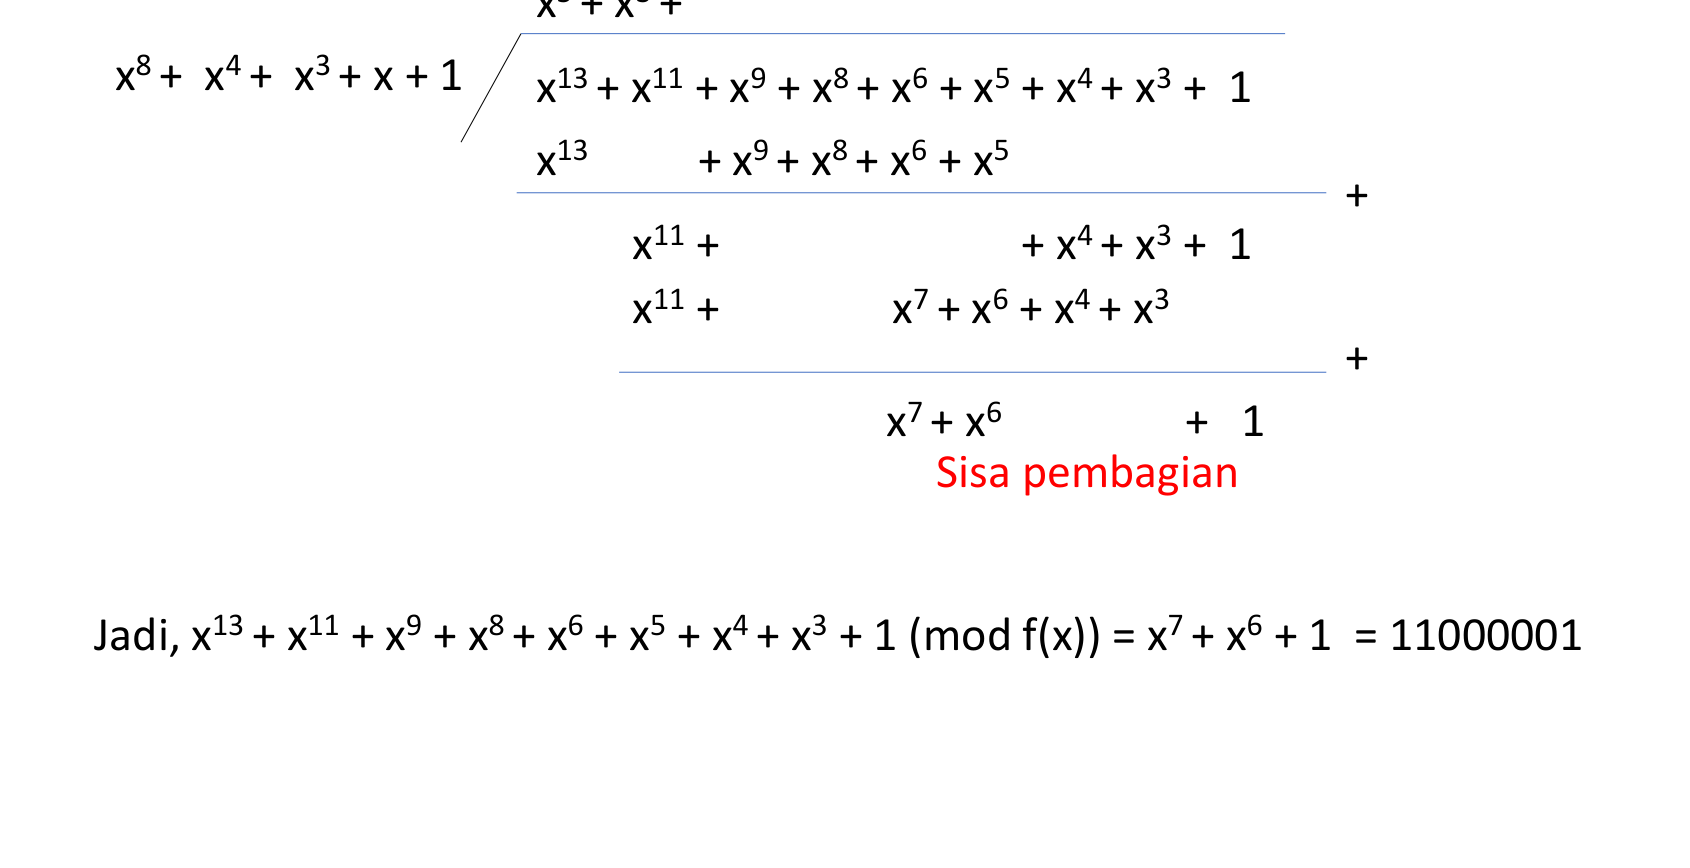
\includegraphics[width=0.62\linewidth, height=0.65\textheight, keepaspectratio]{figures/pembagian-polinom.png}
    \caption{Pembagian panjang polinom di dalam $GF(2)$: hasil kali
    $x^{13} + x^{11} + x^9 + x^8 + x^6 + x^5 + x^4 + x^3 + 1$ dibagi oleh
    $x^8 + x^4 + x^3 + x + 1$ untuk memperoleh sisa $x^7 + x^6 + 1$}
    \label{fig:pembagian-polinom}
    \sumber{Munir, \textit{IF4020 Kriptografi}, ITB.}
\end{figure}

Contoh ketiga memakai medan yang lebih kecil agar seluruh pembagiannya dapat
diikuti dengan mata. Misalkan $a = x^3 + x^2 + 1$ dan $b = x^2 + x$, keduanya di
dalam $GF(2^4)$ dengan polinom tereduksi $x^4 + x + 1$. Hasil kali mentahnya
adalah
\[
(x^3 + x^2 + 1)(x^2 + x) = x^5 + x^4 + x^4 + x^3 + x^2 + x
= x^5 + x^3 + x^2 + x ,
\]
yang dalam biner ditulis $\code{101110}$. Karena hasilnya berderajat lima,
ia direduksi oleh $x^4 + x + 1$. Pembagiannya hanya memerlukan satu langkah:
$x^5$ dibagi $x^4$ menghasilkan $x$, dan
\[
x \cdot (x^4 + x + 1) = x^5 + x^2 + x .
\]
Mengurangkan (yakni meng-XOR-kan) hasil itu dari polinom semula:
\[
(x^5 + x^3 + x^2 + x) \oplus (x^5 + x^2 + x) = x^3 .
\]
Sisa $x^3$ sudah berderajat tiga, lebih kecil daripada $m = 4$, sehingga
prosesnya berhenti. Jadi $a \cdot b = x^3 = \code{1000}$.

Perlu ditegaskan satu hal yang sering menimbulkan salah paham. Tidak setiap
polinom berderajat rendah bersifat tereduksi, dan tidak setiap polinom yang
tampak rumit bersifat tereduksi. Polinom $x^4 + x + 1$ \emph{tidak dapat
direduksi} di dalam $GF(2)$: ia tidak punya akar ($0 \mapsto 1$ dan
$1 \mapsto 1$), dan satu-satunya polinom kuadratik tak tereduksi di $GF(2)$
adalah $x^2 + x + 1$, yang kuadratnya $x^4 + x^2 + 1$ berbeda dari $x^4 + x + 1$.
Sebaliknya, polinom $x^2 + 1$ \emph{dapat} direduksi di dalam $GF(2)$, sebab
$(x + 1)^2 = x^2 + 2x + 1 = x^2 + 1$. Kenyataan itu memperlihatkan bahwa
polinom yang tak tereduksi di atas bilangan riil belum tentu tak tereduksi di
dalam $GF(2)$; kriterianya bergantung sepenuhnya pada medan tempat polinom itu
berada.

\subsection{Mengapa ECC Memerlukan Medan Berhingga}
\label{subsec:mengapa-medan}

Kurva eliptik dapat didefinisikan di atas bilangan riil, dan di sanalah
geometrinya paling mudah dipahami melalui gambar. Namun bilangan riil tidak
layak dipakai untuk kriptografi, dan alasannya bukan sekadar soal estetika.
Komputer menyimpan bilangan riil dengan jumlah bit terbatas, sehingga setiap
hasil operasi dibulatkan. Kesalahan pembulatan itu menumpuk seiring operasi
yang berantai, dan setelah puluhan perkalian skalar, dua perhitungan yang
seharusnya menghasilkan titik yang sama justru menghasilkan dua titik yang
berbeda tipis. Penerima yang sah tidak dapat memulihkan pesan, bukan karena
penyerang menghalanginya, melainkan karena mesinnya sendiri kehilangan
ketepatan.

Kriptografi menuntut kepastian, bukan ketepatan hampiran. Karena itu semua
pekerjaan harus berlangsung di ranah bilangan bulat, di mana setiap operasi
memberi jawaban yang tepat sama di setiap mesin. Inilah alasan kurva eliptik
untuk kriptografi didefinisikan di atas medan berhingga, yakni $GF(p)$ atau
$GF(2^m)$. Pada medan semacam itu, setiap operasi --- termasuk pembagian yang
muncul di dalam rumus gradien --- merupakan operasi modular yang hasilnya
selalu bulat, tunggal, dan dapat diperiksa ulang. Bab ini membatasi diri pada
kurva eliptik di atas $GF(p)$, sedangkan aritmetika $GF(2^m)$ di atas
menyediakan perkakas untuk memahami varian biner yang dipakai banyak
implementasi perangkat keras.

Dengan perkakas aljabar itu lengkap, bagian berikutnya menyusun objek
utamanya: himpunan titik yang membentuk kurva eliptik, beserta aturan
penjumlahannya.
